% Template by Falko Galperin <falko1@tzi.de>, 2022, V1.0
% Main styling of the template comes from the ClassicThesis package by André Miede.

% IMPORTANT POINTS BELOW:
% - Look at the options between "CONFIGURATION HERE" and "CONFIGURATION ENDS".
% - Abstract.tex contains the abstract (can be disabled).
% - Inhalt.tex contains the contents of your thesis.
% - Glossar.tex contains the glossary (can be disabled) and further options.

% Less important points:
% - You can compile a PDF using `make` and clean up unnecessary files 
%   using `make clean`. `make pdf` combines both.
% - CMYK color space will be used so that printers don't get confused.
% - Feel free to configure other parts outside of the section below too,
%   e.g. uncomment the list of tables if you want that.

%%% CONFIGURATION HERE %%%

% Enter information about your thesis here, adjust as necessary.
% I recommend keeping the `\xspace` at the end.
\newcommand{\myTitle}{System porting to mobile devices at the example of the SEE project\xspace}
\newcommand{\mySubtitle}{Master Thesis\xspace}
\newcommand{\myName}{Roman Gressler\xspace}
\newcommand{\myNumber}{3217822\xspace}
\newcommand{\myProf}{Prof.\ Dr.\ Rainer Koschke\xspace}
\newcommand{\myOtherProf}{Prof.\ Dr.\ Zwetachter\xspace}
\newcommand{\myDepartment}{Faculty 3 --- Mathematics and Computer Science\xspace}
\newcommand{\myDegree}{Computer Science\xspace}
\newcommand{\myDate}{\today}
\newcommand{\myVersion}{\classicthesis}

% Whether links should be colored.
\def\colorLinks{true}

% Color for citations.
\def\citeColor{Periwinkle}

% Color for URLs.
\def\urlColor{Cyan}

% The file in which your BibLaTeX sources reside.
% Remove this line to disable the bibliography.
\def\sourcesFile{sources.bib}

% If you won't use the glossary template, remove the following line.
% Otherwise, set this to the filename of the glossary LaTeX file.
\def\glossaryFile{Glossar.tex}

% If you don't want to have an abstract, remove the following line.
% Otherwise, set this to the filename of the LaTeX file containing the abstract.
\def\abstractFile{Abstract.tex}

% Despite the seemingly broad implications of this option, it'll simply include a 
% disclaimer for readers in case you don't want to use something 
% like the "Gendersternchen". Set it to 1 to enable this disclaimer.
\def\disableGender{0}

% Set this to 1 if you want to use \section for the highest level of headings.
% Otherwise, \chapter will be used.
% IMPORTANT NOTE: This template assumes this value will be 1.
% If you choose to set it to something other than 1, you'll need to
% adjust this template's usage of \section and change it to \chapter.
\def\disableChapter{1}

% These are ClassicThesis options. 
% Don't forget to set drafting=false for the final version.
% If you have pdflatex, I recommend eulermath=true, it looks a bit better in my opinion.
\PassOptionsToPackage{
  drafting=true,  % print version information on the bottom of the pages
  tocaligned=false, % the left column of the toc will be aligned (no indentation)
  dottedtoc=true,  % page numbers in ToC flushed right
  eulerchapternumbers=true, % use AMS Euler for chapter font (otherwise Palatino)
  linedheaders=false,  % chaper headers will have line above and beneath
  floatperchapter=true,  % numbering per chapter for all floats (i.e., Figure 1.1)
  eulermath=false,  % use Euler fonts for mathematical formulae (only with pdfLaTeX)
  beramono=true,    % toggle a different monospaced font (w/ bold)
  style=classicthesis % classicthesis, arsclassica
}{classicthesis}

%%% CONFIGURATION ENDS %%%
% (Of course, feel free to modify the rest of the below code too.)

% ClassicThesis causes these false positive warnings, hence we silence them.
\RequirePackage{silence} % :-\
    \WarningFilter{scrreprt}{Usage of package `titlesec'}
    \WarningFilter{titlesec}{Non standard sectioning command}

\documentclass[twoside,openright,titlepage,numbers=noenddot,%headlines,
               headinclude,footinclude,cleardoublepage=empty,abstract=on,
               BCOR=5mm,paper=a4,listof=totocnumbered]{scrreprt}
\usepackage[utf8]{inputenc}
\usepackage[T1]{fontenc}

\PassOptionsToPackage{hyphens}{url}

\usepackage[ngerman]{babel}
\usepackage[dvipsnames,usenames,cmyk]{xcolor}
\usepackage{hyperref} 
\usepackage{xspace}
% \usepackage[style=alphabetic]{biblatex}
\usepackage[round]{natbib} % Literatur und Referenzen
\usepackage{bm}
\usepackage{dsfont}
\usepackage{sidenotes}
\usepackage{newpxtext}
\usepackage{epigraph}
\usepackage{etoolbox}
\usepackage{multicol}
\usepackage{graphicx}
\usepackage{wrapfig}
\usepackage{microtype}
% Note: If you enable this, you need the -shell-escape flag.
%\usepackage{minted}
%\usemintedstyle{friendly}
\usepackage{xifthen}
\usepackage{enumitem}
\usepackage{calc}
\usepackage{subfig}
\usepackage{amssymb}
\usepackage{scalerel}
\usepackage[noend]{algpseudocode}
\usepackage{algorithm}
\usepackage{xstring}

\usepackage[normalem]{ulem}
\setlength{\columnsep}{0,1cm}

\usepackage{classicthesis}
\usepackage{titlesec}

% Make headings a little more discernable.
\titleformat*{\chapter}{\LARGE\bfseries}
\titleformat*{\section}{\Large\bfseries}
\titleformat*{\subsection}{\large\bfseries}

\hypersetup{colorlinks=\colorLinks, citecolor=\citeColor, 
    urlcolor=\urlColor, linktocpage=true, bookmarksnumbered,
  pdftitle={\myTitle},%
  pdfauthor={\textcopyright\ \myName, University Bremen},%
  pdfsubject={\mySubtitle},%
  pdfcreator={pdfLaTeX},%
  pdfproducer={LaTeX with classicthesis and FG-V1.0}%
}

%\ifdef{\sourcesFile}{\addbibresource{\sourcesFile}}{}

% Allow " instead of "` and "'
\usepackage{csquotes}
\MakeOuterQuote{"}

% Uncomment this if you want textsc to be a little (x 1.15) bigger.
%\usepackage{letltxmacro,scalefnt}
%\newcommand{\bigtextsc}[1]{\textsc{\scalefont{1.15}#1}}

% Some custom commands:
% Proper spacing for "z.B."
\newcommand{\zB}{z.\,B.\xspace}
% Command for TODOs, use either \TODO or \TODO{Details}
\newcommand{\TODO}[1]{\textbf{\textcolor{red}{\ifthenelse{\isempty{#1}}{TODO!}{TODO: #1}}}\xspace}
% Properly color Axivion's name.
\newcommand{\Axivion}{\textsc{{\color{black}{A}}{\color{red}{x}}{\color{black}{ivion}}}}

\newcommand{\Regie}[1]{\textbf{Regie:} #1}
\newcommand{\Stil}[1]{\textbf{Stil:} #1}

% Improve caption fonts.
\setkomafont{caption}{\footnotesize\itshape}
\setkomafont{captionlabel}{\usekomafont{caption}}

% Import glossary if necessary.
\ifdef{\glossaryFile}{\input{\glossaryFile}}{}

\begin{document}

\title{\myTitle}
\subtitle{\mySubtitle}
\author{\myName}
\date{\myDate} 

\raggedbottom
\selectlanguage{ngerman}
\captionsetup[subfigure]{justification=centering}

\pagestyle{plain}
\pagenumbering{roman}

\begin{titlepage}
    \begin{addmargin}[-1cm]{-3cm}
	\begin{center}
		\Huge
		\vspace*{1cm}
        \begingroup
            \myTitle \\ \bigskip
        \endgroup
		\LARGE
        \mySubtitle\\
		\vspace{3cm}
 		\Large
		\myName\\
		\vspace{6pt}
        Matriculation number: \myNumber\\
		\vspace{1cm}
		\myDate\\
		\vspace{2cm}
 		
\includegraphics[width=6cm]{unibremen}\\
 		\vspace{1cm}
 		\large
 		\myDepartment\\
		\myDegree\\
		\vspace{4cm}
		\large
		1. Supervisor: \myProf\\
		2. Supervisor: \myOtherProf\\
		\vspace{1.5cm}
	\end{center}
    \end{addmargin}
\end{titlepage}
\cleardoublepage{}

\ifdef{\abstractFile}{%
\pdfbookmark[1]{Zusammenfassung}{abstract}
\chapter*{Zusammenfassung}
\input{\abstractFile}
\cleardoublepage{}
}{}

\pdfbookmark[1]{Erklärung}{erklaerung}
\chapter*{Erklärung}\label{erklaerung}
Ich versichere, diese Arbeit --- sofern dies nicht explizit anders
gekennzeichnet wurde --- ohne fremde Hilfe angefertigt zu haben.  Ich
habe keine anderen als die angegebenen Quellen und Hilfsmittel
benutzt.  Alle Stellen, die wörtlich oder sinngemäß aus
Veröffentlichungen entnommen sind, sind als solche kenntlich gemacht.

\bigskip

\noindent\textit{Bremen, den \today}
\smallskip
\begin{flushright}
    \begin{tabular}{m{5cm}}
        \\ \hline
        \centering\myName \\
    \end{tabular}
\end{flushright}

\vfill

\cleardoublepage{}

\pdfbookmark[1]{Danksagung}{Danksagung}
\begingroup
\let\clearpage\relax
\let\cleardoublepage\relax
\let\cleardoublepage\relax
\chapter*{Danksagung}
\TODO{Danksagung hier.}


\ifdef{\disableGender}{%
\if\disableGender1
\vfill
\chapter*{Gender-Hinweis}
Aus Gründen der besseren Lesbarkeit wird auf die gleichzeitige
Verwendung der Sprachformen männlich, weiblich und divers verzichtet.
Sämtliche Personenbezeichnungen gelten gleichermaßen für alle
Geschlechter.

\vfill
\fi
}{}
\endgroup

\cleardoublepage

\pagestyle{scrheadings}

% Table of contents:
\pdfbookmark[1]{\contentsname}{tableofcontents}
\tableofcontents

\clearpage

\ifdef{\disableChapter}{
\if\disableChapter1
\let\subsubsection\subsection
\let\subsection\section
\let\section\chapter
\fi}{}

\cleardoublepage
\pagenumbering{arabic}

\section{Concept}
\label{section:concept}
In this section a concept of a mobile \gls{see} version will be presented. 
Therefore, a prototype will be created to point out the features that a mobile version of \gls{see} requires.

Prototypes are a common way to express the needs of a system. 
It is a low-cost way of planning an implementation, that can highlight challenges regarding constraints of a system early on.

Even though a prototype will never be able to show every aspect and need of a complex system, it should still help to answering questions like: 
How should the system feel? How should it be implemented, and what are the key features? \cite{houde1997prototypes} 

\gls{see} is meant to be used by multiple platforms such as desktop devices, mobile devices and virtual reality devices.
Each device has different interaction constrains. 
While a desktop user will control the player with mouse and keyboard a mobile user will interact with virtual joysticks on a touchscreen.
Selecting nodes of a \gls{city} will be done by clicking it with a mouse on desktop devices, while a mobile device will require a touch input.

\subsection{Interface}

In the following a paper prototype will be presented that marks out a concept for the mobile interface.
Since the field of mobile development is quite young there few guidelines regarding the design of mobile device interfaces.
A guideline that is widely accepted is problematic to find. \cite{renaud2017demarcating}, \cite{punchoojit2017usability}

Major differences to desktop environments are the screen size, forms of input and input feedback.
To assure as much space is used for the actual interaction of the app the menu should just take as much space as needed.
As a study has found out, a size of at least 8*8 mm is needed to reduce error rates selecting the right button. \cite{conradi2015optimal} \cite{parhi2006target}
TODO WEITER AUSFÜHREN
SHORTCUTS WIE STRG Z NICHT MÖGLICH
 \cite{adipat2005interface} 

Moving the player will be handled with virtual joysticks as seen in figure \ref{fig:joystick}.
The left joystick will move the player through the virtual room and the right will move the camera angle or in other word the direction the player looks at.
The joysticks are placed in the left and right corner and should just take as much space as needed to be handled comfortably.
This way the player is able to navigate through the virtual room with his/her thumps while still having enough space to work on the \gls{city}.

\begin{figure}[htb]
    \centering
    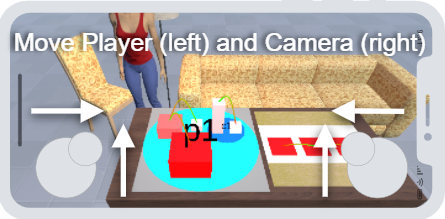
\includegraphics[width=1\textwidth]{Concept/img/joystick.png}
    \caption{Joysticks for moving in \gls{see}}\label{fig:joystick}
\end{figure}

The menu on the top left side seen in figure \ref{fig:quickbar} will be called "quickbar" further on. 
The quickbar can be minimized to safe screen space when not needed. 
The quickbar is designed to offer more general functions that are needed in various situations.
Because there are no shortcuts on mobile devices each function has to have a button to be activated.

The functions are redo and undo which will do an action undone again or revert an action.
Then there is a camera lock that will lock the players perspective to a certain \gls{city} so that the player can only move around the selected city and move closer or further away from it.
The next function is to rerotate a \gls{city}.
That means the \gls{city} that was last rotated will be set back to its initial state of rotation.
Last but not least there will be a button for recentering the city, which will work quite similar to the rerotate button and center the last moved \gls{city}.
The button on the right can be used to collapse or expand the quickbar.
\begin{figure}[htb]
    \centering
    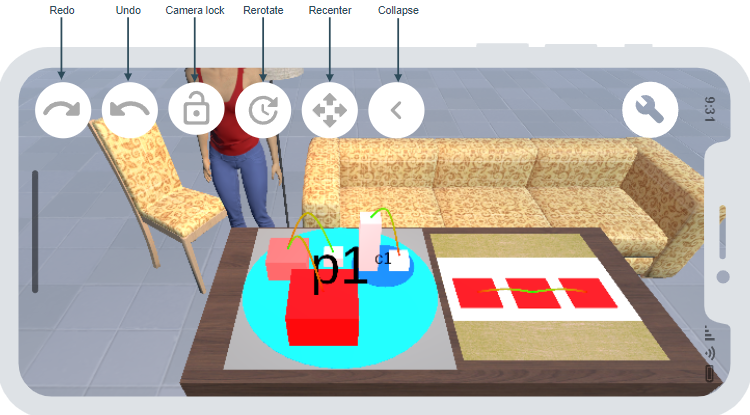
\includegraphics[width=1\textwidth]{Concept/img/quickbar.png}
    \caption{Quickbar for various interactions in \gls{see}}\label{fig:quickbar}
\end{figure}

On the top right side another menu will be placed that contains different interaction modes.
By clicking a button an interaction mode will be selected and moved to the top right corner.
Also, the menu will be collapsed and only the buttons regarding the selected interaction mode shall be shown.
By clicking the button on the top right again the menu shall expand and the other interaction modes shall be selectable.
The other buttons shall be kept in the same order to reduce confusion of the user.

The first interaction mode, seen in figure \ref{fig:select}, is for selecting nodes.
Nodes can be selected by being touched and deselected by being touched again.
There can be multiple nodes selected at once.
The hole selection can be deselected by clicking the deselect button next to the select interaction mode button.
Selected nodes shall be highlighted with a different node color and also display their name.

\begin{figure}[htb]
    \centering
    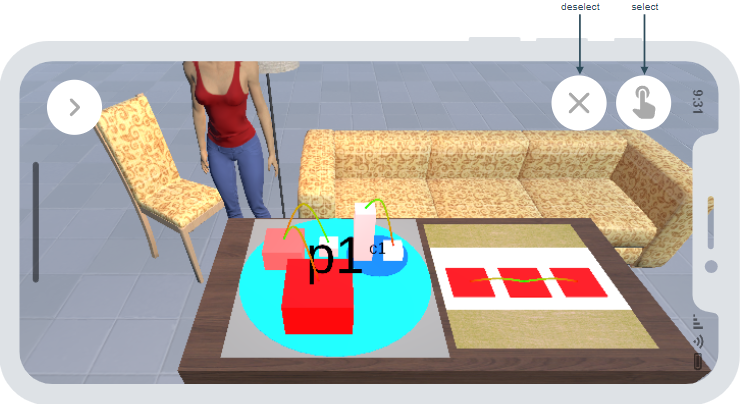
\includegraphics[width=1\textwidth]{Concept/img/menu1.png}
    \caption{Selection mode in \gls{see}}\label{fig:select}
\end{figure}

The second interaction mode, seen in figure \ref{fig:delete}, is for deleting node.
It does not need additional buttons.
Node will be deleted by being touched.-
Unlike in the desktop version there will not be a group deletion interaction because it would require an additional menu panel.
The added functionality would be minimal and selecting a group of nodes, confirming and finally deleting would require a handful more steps and would therefore most likely not be used.

\begin{figure}[htb]
    \centering
    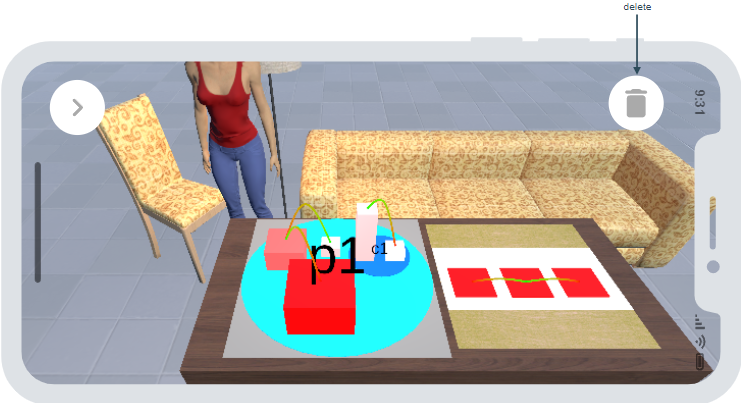
\includegraphics[width=1\textwidth]{Concept/img/menu2.png}
    \caption{Delete mode in \gls{see}}\label{fig:delete}
\end{figure}

The following interaction mode, seen in figure \ref{fig:nodes}, is dedicated to the nodes and edges of a \gls{city}.
Starting on with the "add node" button on the right.
When activated the user can create new node by clicking on a certain spot on the \gls{city} plane. 
The following button on the left is for adding edges.
By selecting two nodes a new edge will be created between them. 
Then, the button one further on the right is for editing nodes.
By touching a node a window will pop up that allows the user to edit the node by changing its name and its type.
Last but not least the button on the left-hand side will be used to scale nodes.
That means the node height and width can be adjusted by first selecting it via touch and then hold a corner and slide it further away from the node center to increase the size or slide it towards the center to decrease the size of the node.
Each button of the node interactions will be marked green after being pressed to indicate that it is active.

\begin{figure}[htb]
    \centering
    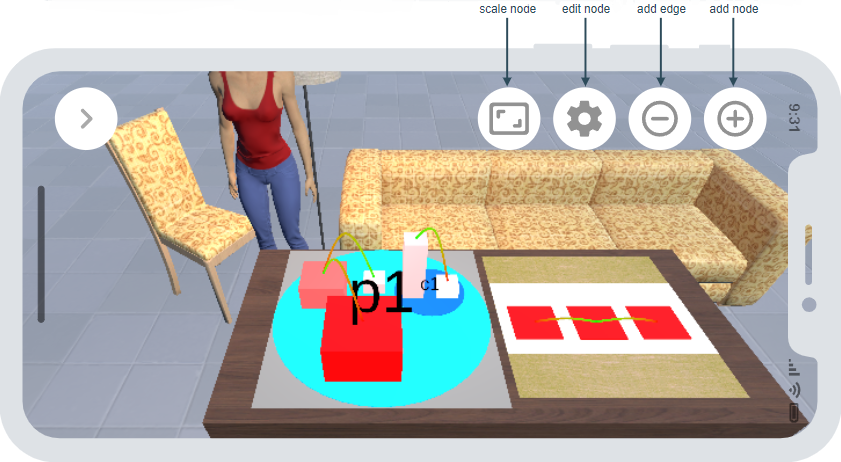
\includegraphics[width=1\textwidth]{Concept/img/menu3.png}
    \caption{Node interactions in \gls{see}}\label{fig:nodes}
\end{figure}

Then there will be a button for rotation interactions that can be seen in figure \ref{fig:rotate}.
Starting with the first activatable button that lets the user rotate the hole \gls{city} by touching any point on it and then sliding away from that point.
Similar to that there will be a button that lets the user rotate just a single node on the \gls{city}.
In addition to that there will be a button that activates the so-called "locked-rotation" mode.
While in "locked-rotation" mode the rotation of a node or \gls{city} will be done in eight predefined steps to a full rotation.
Each step will have the same 45° range.
The last button of this group will be for changing the center of the rotations. 
There are to options: the first option is a center of rotation in the middle of the \gls{city} and the second is in the middle of a node selection made with the interactions seen in figure \ref{fig:select}.
The second option can be activated by pressing the last button.

\begin{figure}[htb]
    \centering
    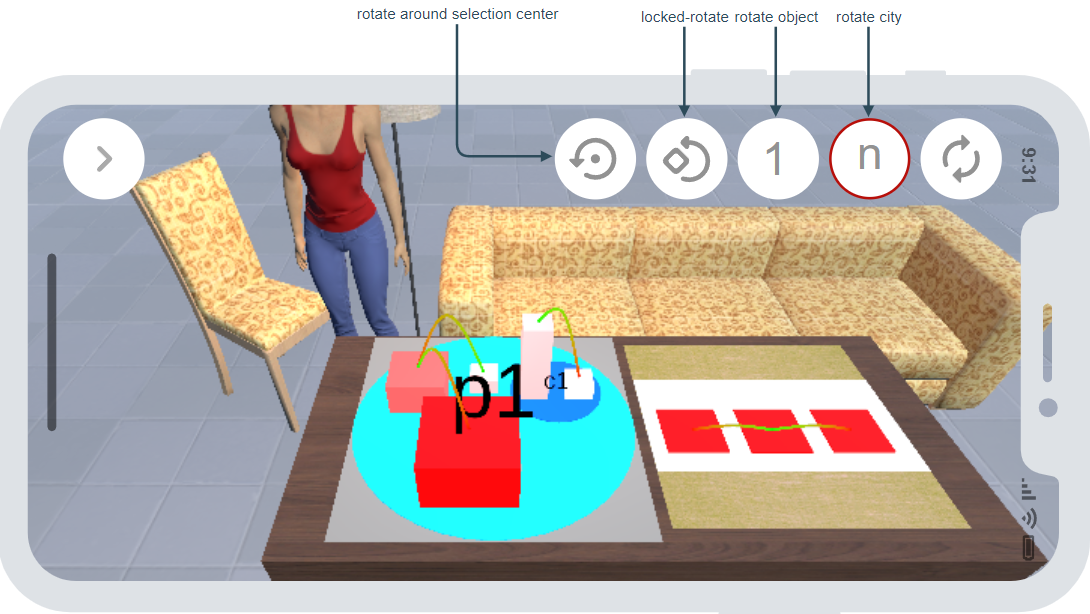
\includegraphics[width=1\textwidth]{Concept/img/menu4.png}
    \caption{Rotation mode in \gls{see}}\label{fig:rotate}
\end{figure}

The last interaction group, seen in figure \ref{fig:move}, is for moving the \gls{city} or a single node.
The move interactions are quite similar to the rotation interactions.
There will be a button to move a hole \gls{city} as well as a button to move only single nodes.
In addition to that there will be a button that restricts the movement of the \gls{city} or node to a predefined direction.
The directions will be again in 45° angles and objects can be moved on a straight line on that angle.
Moving a node or a \gls{city} can be achieved by touching and holding it and then moving it to the desired position.
\begin{figure}[htb]
    \centering
    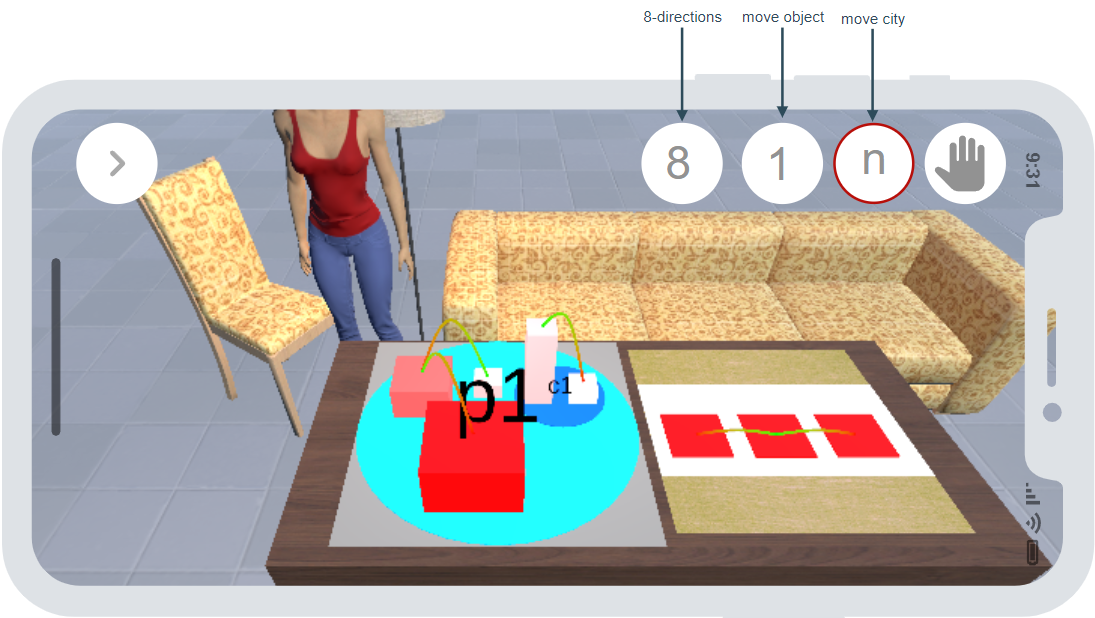
\includegraphics[width=1\textwidth]{Concept/img/menu5.png}
    \caption{Movement mode in \gls{see}}\label{fig:move}
\end{figure}

\subsection{Interaction}

Smartphones are quite limited in space and there are few input possibilities.
Unlike a desktop computer there is no mouse and there is no physical keyboard.
Smartphones use virtual keyboards but due to the restriction of screen space the keyboard is hidden most of the time.
Which would make keyboard shortcuts uncomfortable because the user has to open the keyboard first.
Therefore, smartphones need different ways of interaction such as touch gestures. 

Zooming in to a \gls{city} happens by scrolling on a desktop environment. 
The is no option to scroll on mobile devices, but there are at least two popular alternatives.
The first option would be to double tap on the \gls{city} to zoom in.
The double tap would zoom in, in predefined steps and after reaching a certain level of closeness it would trigger to zoom out again.
In \gls{see} zooming in, in predefined steps might not be precise enough because there could be a quite large \gls{city} or a rather small one.
Finding predefined steps that would fit every situation is rather hard.
Therefore, a second option by zooming in with a two finger gesture might be better. 
In this option the user uses two fingers and slides them towards each other to zoom in or slides the two fingers away from each other to zoom out.
This way there are no predefined steps necessary and zooming interactions can be done precisely.
\subsection{Requirements}
In the following a list of requirements will be given, which will specify in detail what the implementation of a mobile version has to take care of.
The list will be referred to multiple times in the upcoming realization part in chapter \ref{section:implementation}.
Requirements are essential for the planning phase as they give a good fundamental structure for the developer to rely on. \cite{Robertson2012,Stevens2005}
\begin{itemize}
    \item[{[R1]}] The application shall run on Android devices
    \item[{[R2]}] The application shall be controlled via touchscreen
    \begin{itemize}
        \item [{[R2.1]}] The player and camera shall be moved with virtual joysticks
        \item [{[R2.2]}] Needed shortcuts of the desktop version shall be handled with buttons
        \item [{[R2.3]}] Zooming shall be handled with a two finger gesture
    \end{itemize}
    \item[{[R3]}] The user shall be able to select a node of a \gls{city}
    \begin{itemize}
        \item [{[R3.1]}] After selecting the name of the node shall be shown
        \item [{[R3.2]}] The user shall be able to deselect single nodes or a group of nodes
    \end{itemize}
    \item[{[R4]}] The user shall be able to delete nodes
    \item[{[R5]}] The user shall be able to interact with nodes
    \begin{itemize}
        \item [{[R5.1]}] The user shall be able to add nodes
        \item [{[R5.2]}] The user shall be able to add edges
        \item [{[R5.3]}] The user shall be able to edit nodes
        \item [{[R5.4]}] The user shall be able to scale nodes
    \end{itemize}
    \item[{[R6]}] The user shall be able to rotate a \gls{city}
    \begin{itemize}
        \item[{[R6.1]}] The user shall be able to rotate a \gls{city} in 45° steps
        \item[{[R6.2]}] The user shall be able to rotate single objects
        \item[{[R6.3]}] The user shall be able to rotate around a center of selected nodes
        \item[{[R6.4]}] The user shall be able to undo the rotation
    \end{itemize}
    \item[{[R7]}] The user shall be able to move a \gls{city}
    \begin{itemize}
        \item[{[R7.1]}] The user shall be able to move single object of a \gls{city}
        \item[{[R7.2]}] The user shall be able to restore the \gls{city} initial position
        \item[{[R7.3]}] The user shall be able to move a \gls{city} or single node in predefined directions
    \end{itemize}
    \item[{[R8]}] The user shall be able to undo and redo actions
    \item[{[R9]}] The user shall be able to lock the camera to a selected \gls{city}
\end{itemize}
\section{Einführung}

\Regie{Diese Vorlage ist aufgeteilt in die Kapitel Einführung,
  Grundlagen und verwandte Arbeiten, Konzept, Umsetzung, Evaluation,
  Zusammenfassung und Ausblick. Das ist eine generische, klassische
  Aufteilung. In Einzelfällen kann auch eine andere Aufteilung
  vorgenommen werden, aber letztlich muss zu all diesen Punkten etwas
  in der Arbeit gesagt werden. Auch die Titel der Kapitel können
  eventuell angepasst werden.} 

\Regie{Ein allgemeiner Hinweis: Eine Abschlussarbeit als
  wissenschaftliche Arbeit hat immer zwei Ebenen: Auf der konkreten
  Ebene wird transparent dargestellt, was gemacht wurde. Auf der \glqq
  Metaebene\grqq{} wird reflektiert, warum man das und nicht etwas
  Anderes gemacht hat. Hierzu werden also Alternativen explizit
  genannt und gegeneinander abgewogen. Es wird begründet, warum man
  sich dann für das konkrete Vorgehen entschieden hat.}
  
\Regie{In der Einführung wird die Aufgabenstellung präzise formuliert
  und geeignet motiviert.  Danach folgt eine kurze Übersicht über den
  Rest des Dokuments.}

\Regie{Bitte gleich zum Punkt kommen. Bei der Motivation nicht erst
  langatmig ausholen, wie komplex und allgegenwärtig Software ist. Das
  wissen die Gutachter(innen) und haben es schon viel zu oft nochmals
  lesen müssen.}

\Stil{Zwischen einer Überschrift und seines ersten Unterabschnitts
  muss ein kurzer Text kommen. Zum Beispiel kann man hierin
  beschreiben, was den Leser in diesem Kapitel erwartet.}

\Stil{Ganz am Ende, wenn das Dokument fertig zu sein scheint und man
  es eigentlich nur noch ausdrucken möchte, dann möge man bitte zuvor
  noch einmal das Inhaltsverzeichnis ansehen. Dort ist zu prüfen, ob
  bei einer Unterteilung eines Abschnittes auch immer mindestens zwei
  solche Unterteilungen existieren. Immer wieder kommt es vor, dass es
  beispielsweise einen Unterabschnitt 2.3.1, aber keinen
  Unterabschnitt 2.3.2 gibt.  Wenn es nur einen Unterabschnitt gibt,
  dann ergibt eine Unterteilung keinen Sinn.}

\Stil{Bitte auf die Rechtschreibung achten. Viele Arbeiten enthalten
  viel zu viele Fehler. Die Schreibweise von Worten kann man
  nachschlagen. Es gibt Tools, die einfache Tippfehler erkennen. Es
  gibt Regeln für Kommata. Rechtschreibung kann man lernen.  Es gibt
  keine Ausrede für mangelhafte Rechtschreibung, wenn man nicht an
  Legasthenie leidet.  Natürlich werden immer einige Fehler schlicht
  übersehen werden, wenn es aber zu viele davon gibt, stört das den
  Lesefluss und macht den schlechten Eindruck mangelnder Sorgfalt.
  Man sollte immer eine andere Person, die sicher in der
  Rechtschreibung ist, bitten, das Dokument durchzulesen, weil man
  sich seiner eigenen Fehlern vielleicht nicht bewusst ist.  Es eignet
  sich dafür eine Person besonders gut, die vom Inhalt selbst gar
  nicht viel versteht und sich allein auf die Form konzentrieren
  kann.}

\Stil{Fußnoten sollten möglichst vermieden werden, weil sie den Leser
  zwingen, den Kontext zu wechseln. Will man einen Artikel
  referenzieren, dann nimmt man ohnehin eine Zitierung; siehe
  unten. Ansonsten verwendet man Klammern oder Gedankenstriche, um den
  Text direkt in den Lesefluss einzubetten. Und vielleicht ist das,
  was man in die Fußnote packen möchte, ohnehin irrelevant, dann kann
  man es auch ganz weglassen. Wenn man etwas in eine Fußnote steckt,
  muss man sowieso damit rechnen, dass es keiner liest.}
  
\section{Grundlagen und verwandte Arbeiten}

\Regie{Hier werden alle wesentlichen und nur die wesentlichen
  Grundlagen, die nicht als bekannt vorausgesetzt werden können,
  aufgeführt. Manchmal liest man Arbeiten, die den Mangel an eigenem
  Beitrag mit einem überbordenden Grundlagenkapitel zu kompensieren
  versuchen. Bei allem, was hier beschrieben wird, stets kritisch
  reflektieren, ob erstens davon auszugehen ist, dass den
  Gutachter(innen) das bereits nicht schon zur Genüge bekannt sein
  dürfte, und zweitens, ob das in einem späteren Kapitel auch wirklich
  wieder aufgegriffen wird.}

\Regie{Bachelor- und Masterarbeiten sind wissenschaftliche
  Abschlussarbeiten. Demzufolge gehört es auch dazu, dass man sich mit
  der wissenschaftlichen Literatur auseinandergesetzt hat. Man sollte
  dabei keineswegs nur die Literatur einfach nur wiedergeben, sondern
  sich auch kritisch mit ihr auseinandersetzen. Insbesondere ist
  darzulegen, wie Aspekte der gesichteten Literatur Einfluss auf die
  eigene Arbeit genommen haben. Zur Frage, wie man Literatur
  systematisch sucht und zusammenfasst, gibt es in der Literatur eine
  Reihe von Empfehlungen \citep{Kitchenham:TR:07, Brereton:JSS:07,
    Petersen:EASE:08, Kitchenham:IST:09, Wohlin:JSS:13,
    Kitchenham:EASE:10, Petersen:IST:15}. Insbesondere der technische
  Bericht von \cite{Kitchenham:TR:07} stellt eine ausführliche
  Anleitung dar.}

\Stil{Wobei wir beim Zitierstil wären. Für Zitierungen gibt es im
  Deutschen tatsächlich eine Norm: die DIN 1505. Hier werden die
  Autoren -- zumindest partiell -- und die Jahreszahl für die
  Zitierung verwendet. Das ist zwar länglicher als reine Nummern oder
  kryptische Abkürzungen, wie sie gerne in Aufsätzen mit wenig Platz
  benutzt werden, enthält aber mehr lesbare und erinnerbare
  Informationen. Außerdem kann man sie besser in den Satz einbauen,
  wie es oben schon beim Verweis auf den Bericht von
  \cite{Kitchenham:TR:07} gezeigt wurde.}

% Das Folgende ist nur zur Demonstrieren.
% Lösch ruhig erstmal alles aus dieser Datei, sobald du mit der Arbeit anfängst.

\if\disableChapter1
\subsection{Glossarbeispiel}
\ifdef{\glossaryFile}{ Es können auch Glossarbegriffe verwendet werden
  (falls Glossar.tex so konfiguriert wurde), im Kontext von \gls{see}
  könnte man \zB{} über \glspl{city} reden wollen.
  \if\defineOnFirstUse1 Du siehst, wie die neuen Begriffe als
  \texttt{\detokenize\expandafter{\firstUseCommand}}angezeigt werden.
  \else Du hast kein \verb+\firstUseCommand+ festgelegt, deswegen
  werden die Begriffe ohne ihre Definition abgedruckt (die ist
  natürlich aber trotzdem im Glossar).
  \fi%
  Für mathematische Glossarbegriffe würde man das so machen:
  $\glssymbol{S}_{\emptyset} = \{\emptyset\}$. \firstUseSymbol{S}

  Nachdem man jetzt den Begriff \enquote{\gls{see}} oder
  \enquote{\gls{city}} schonmal verwendet hat, wird er auch ganz
  normal angezeigt (ist aber immer noch anklickbar).  Wenn die
  Glossarbegriffe irgendwie komisch sind oder kein Glossar auf den
  folgenden Seiten erscheint, führe auf der Kommandozeile
  \texttt{makeglossaries Arbeit} aus.}{Du hast kein Glossar
  definiert, was aber auch nicht schlimm ist.}

\subsection{Abbildungsbeispiel}
\begin{figure}[htb]
    \centering
    
\includegraphics[width=0.7\textwidth]{unibremen}
    \caption{Logo der Universität Bremen.}\label{fig:uni}
\end{figure}

Als Beispiel ist hier in \autoref{fig:uni} das Logo der Uni Bremen.
Wenn du ein etwas breiteres Bild hast, das sich bis in die Ränder
erstrecken soll, verwende statt \verb+\begin{figure}+ einfach
\verb+\begin{figure*}+. Im Moment wird die Abbildung unten
abgedruckt, verwende ansonsten wie üblich
\verb+\begin{figure}[htbp]+ um auch andere Platzierungen zu
erlauben.

Wenn du die Position eines Bilds forcieren willst, würde ich von dem
oft verwendeten Ansatz \verb+\begin{figure}[H]+ abraten, da das manche
Layouts zerschießen kann.  Verwende stattdessen lieber Umgebungen,
die keine Floats sind\footnote{ Siehe bspw.\
\url{https://tex.stackexchange.com/a/8631}.  }, \zB{}
\texttt{minipage} oder einfach \texttt{center}.

\ifdef{\sourcesFile}{ Zitate mit Bib\LaTeX{} funktionieren wie immer,
  als Beispiel hier ein Zitat zum sog.\
  Hawthorne-Effekt~\citep{Hawthorne1939}.  Die Referenzen kommen
  einfach in die \texttt{\sourcesFile}.  }{Du hast scheinbar keine
  Bibliographie eingerichtet, was für eine wissenschaftliche Arbeit
  ungewöhnlich ist. Das solltest du tun. } \else Wenn du das hier
lesen kannst sieht diese Beispielseite vermutlich ziemlich hässlich
aus, weil ich überall \verb+\section+ statt \verb+\chapter+ verwendet
habe.  Ich hab deswegen erstmal die meisten Beispiele entfernt, um es
nicht schlimmer zu machen. Du kannst dir natürlich immer noch einfach
den Quellcode ansehen.  \fi

\vspace{1em}

{\large \emph{Dann viel Erfolg beim Schreiben der Arbeit%
\ifthenelse{\equal{Dein Name\xspace}{\myName}}{}{, {\saveexpandmode\expandarg\StrBefore{\myName}{ }\restoreexpandmode}}!}}

\section{Konzept}

\Regie{Hierin werden die Anforderungen und die Ziele der Arbeit
  nochmals präzisiert und motiviert und Entwurfsentscheidungen
  formuliert, wie diese Ziele durch diese Arbeit erreicht
  werden. Abhängig vom Gegenstand der Arbeit sollten hier auch
  explizit die möglichen Nutzergruppen, dereren Charakteristika und
  Ziele aufgeführt werden. Das letztlich gewählte Konzept sollte nicht
  einfach nur wiedergegeben werden, vielmehr sind auch mögliche
  Alternativen zu nennen und abzuwägen. Es soll nachvollziehbar
  begründet dargelegt werden, warum man sich für genau jenes Konzept
  entschieden hat.}

\section{Umsetzung}

\Regie{Hier wird die Umsetzung (oder auch: Implementierung) näher
  ausgeführt. Sie stellt einen Übergang vom Konzept zum
  implementierten Code dar. Der Code selbst wird im elektronischen
  Anhang oder in Form eines Branches in einem für die Gutachter(innen)
  zugänglichen Repository abgegeben. Die Details des Codes selbst
  gehören somit nicht in die Ausarbeitung. Vielmehr wird die
  Implementierung abstrakter beschrieben. Wenn es nicht-triviale
  Algorithmen zu beschreiben gibt, kann das mit Hilfe von Pseudo-Code
  getan werden. Es können auch UML-Diagramme verwendet werden; diese
  sollten dann bitte auch in korrekter UML-Notation angegeben
  werden. Häufig findet man Klassendiagramme, die einen Überblick über
  die Implementierung geben sollen. Leider sind diese oft so
  umfangreich, dass ihre Abbildung herunterskaliert wird, so dass die
  Texte in den Grafiken nicht mehr lesbar sind. Oft finden sich darin
  Details, auf die im Text gar nicht eingegangen wird, wie (private)
  Attribute und Methoden. Ein Klassendiagramm kann durchaus sinnvoll
  sein, um den Zusammenhang zu erläutern, aber letztlich ist es nur
  ein Bild, das im Text auch erklärt werden muss. Wird etwas davon im
  Text nicht erklärt, ist es entweder irrelevant und kann weggelassen
  werden oder der Text ist nicht vollständig.}

\Regie{Wenn auf anderen Arbeiten aufgebaut wurde, dann muss der eigene
Beitrag deutlich davon abgegrenzt werden. Was wurde übernommen? Was
verändert? Was wurde neu hinzugefügt?}

\Regie{Um das, was man entwickelt hat, besser darzustellen, kann man
  auch noch ein Video drehen. Das bietet sich insbesondere für
  interaktive, graphische Dinge an. Der oder die Zweitgutachter(in)
  wird kaum selbst das entwickelte Programm bauen und ausführen. Für
  diese Person ist es insbesondere hilfreich, wenn sie sich das in
  einem Video vorführen lassen kann.}

\section{Evaluation}

\Regie{Die adäquate Form der Evaluation hängt vom Gegenstand ab,
  insofern wird sich die Darstellung der Evaluation in diesem Kapitel
  von Arbeit zu Arbeit unterscheiden. Allen gemein ist jedoch, dass es
  sich um eine empirische Studie handelt. Egal, ob nur die Laufzeit
  eines Algorithmus gemessen wird oder ob ein kontrolliertes
  Experiment durchgeführt wurde. Bei
  \url{https://seafile.zfn.uni-bremen.de/published/swt/} findet man
  Folien und Videos zur empirischen Softwaretechnik. Dort erfährt man
  viel Nützliches, wie man eine Studie aufbaut und evaluiert.}

\Regie{Die Evaluation muss transparent und nachvollziehbar dargestellt
  werden. Die Ausarbeitung sollte alles so detailliert wiedergeben,
  dass eine andere Person die Studie replizieren kann. Dabei kann für
  sehr detaillierte Aspekte auch auf den Anhang zurückgegriffen
  werden. Dann sollte im Text in diesem Kapitel dennoch eine kurze
  Zusammenfassung dieser Aspekte und der explizite Verweis auf den
  Anhang mit den Details gemacht werden.}
  
\subsection{Forschungsfragen}

\Regie{Hier werden die leitenden Forschungsfragen, die in der
  Evaluation untersucht werden sollen, präzise
  beschrieben. Idealerweise in Form operationalisierter Hypothesen.
  Es wird erläutert, warum diese Forschungsfragen relevant sind.}

\subsection{Versuchsaufbau}

\Regie{Hier wird erklärt, wie die Studie gestaltet ist. Auch wird
  dargelegt, warum der Versuchsaufbau den Forschungsfragen angemessen
  ist, welche Alternativen es gegeben hätte und warum diese verworfen
  wurden. Insbesondere werden hier möglichst vollständig die
  unabhängigen Variablen, die einen Einfluss auf das Versuchsergebnis
  haben können, aufgezählt. Es wird beschrieben, welche davon wie in
  der Studie variiert werden, wenn es sich um ein kontrolliertes
  Experiment handelt. Dann werden vollständig alle abhängigen
  Variablen beschrieben. Sie ergeben sich aus den operationalisierten
  Hypothesen. Die Art und Weise wird präzise beschrieben. Kommen
  hierfür Fragebögen zum Einsatz, wird erläutert, wie der Fragebogen
  zusammengestellt wurde und warum die Fragen relevant sind. Für viele
  Fragestellungen -- insbesondere zur Usability -- gibt es bereits
  Standardfragebögen in der Literatur. Dann sollte man auch auf diese
  zurückgreifen, oder aber überzeugend darlegen, warum diese nicht
  passen. Gibt es mehrere solche Fragebögen, dann werden sie alle
  vorgestellt und gegeneinander abgewogen und einer begründet
  ausgewählt (oder möglicherweise auch mehrere kombiniert).}

\Regie{Der Versuchsaufbau sollte mindestens einmal in einer
  Pilotstudie ausprobiert werden. Damit erzielt man Erkenntnisse, wie
  lange die Probanden später pro Durchlauf brauchen werden und ob sie
  alle gestellten Aufgaben auch tatsächlich verstehen. Die Ergebnisse
  der Pilotstudie können nicht für die Auswertung später verwendet
  werden, weil die Situation eine andere ist und vermutlich sich durch
  die Erfahrungen der Pilotstudie auch noch Änderungen im
  Versuchsaufbau ergeben. Die Erkenntnisse der Pilotstudie und die
  daraus resultierten Änderungen am Versuchsaufbau werden explizit
  genannt.}

\subsection{Probanden und Objekte der Studie}

\Regie{Nehmen an einer Studie Menschen teil, spricht man von ihnen in
  der Regel als Probanden. Nicht sie selbst sind der Gegenstand der
  Untersuchung; vielmehr werden sie benötigt, um etwas untersuchen zu
  können, weil es nicht durch einen Algorithmus automatisiert werden
  kann. Objekte einer Studie sind die Dinge, an denen etwas untersucht
  wird. Das können zum Beispiel Programme sein, in denen die Probanden
  Fehler suchen müssen. Probanden und Objekte sind letztlich auch
  unabhängige Variablen. Das Ergebnis hängt sehr von ihrer Auswahl
  ab. Insofern müssen sie sorgfältig ausgewählt werden, damit die
  Ergebnisse der Studie aussagekräftig und verallgemeinerbar sind. In
  den oben bereits angeführten Videos und Folien zur empirischen
  Softwaretechnik findet man verschiedene Sampling-Methoden, anhand
  derer Probanden und Objekte ausgewählt werden können. Der Einsatz
  systematischer Sampling-Methoden kommt bei den Objekten eher in
  Frage als bei den Probanden. In der Regel kommt realistischerweise
  bei den Probanden nur das Convenience-Sampling zum Einsatz, weil es
  schwierig ist, überhaupt Probanden zu finden, und man in der Regel
  auch nichts über die Gesamtpopulation der Software-Entwicklerinnen
  und -Entwickler weiß. Das ist ein \textit{Threat to Validity} und
  muss offen im Abschnitt~\ref{sec:threats} aufgeführt werden. Um zu
  untersuchen, ob es tatsächlich einen Zusammenhang zwischen
  Eigenschaften der Probanden (\zB{} spezielle Vorkenntnisse mit dem
  Untersuchungsgegenstand oder Programmiererfahrung) gibt, kann man
  auch statistische Untersuchungen zu Korrelation dieser Eigenschaften
  mit den abhängigen Variablen anstellen. In jedem Falle müssen
  relevante Charakteristika sowohl der Probanden (\zB{} Alter,
  Geschlecht, Programmiererfahrung etc.) als auch der Objekte (\zB{}
  Größe und Herkunft der in der Untersuchung verwendeten Programme)
  aufgeführt werden. }

\Regie{Bei der Untersuchung sind auch ethische Fragen und Belange des
  Datenschutzes der Probanden zu berücksichtigen. Dazu sollten vorher
  alle Probanden aufgeklärt worden sein und ein Einverständnis zum
  Datenschutz unterzeichnet haben.}

\subsection{Gestellte Aufgaben}

\Regie{Hier werden die Aufgaben präzise erläutert, die die Probanden
  zu erledigen hatten. Es muss dargelegt werden, warum diese Aufgaben
  repräsentativ für die untersuchten Fragestellungen sind. In der
  Regel sind die Aufgabenbeschreibungen kurz genug, dass man sie hier
  im Text verbatim wiedergeben kann. Sollte das nicht der Fall sein,
  dann kann man sie im Anhang im Detail aufführen und sie hier kurz
  zusammenfassen.}

\subsection{Ergebnisse}

\Regie{Hier werden die quantitativen Ergebnisse wiedergegeben
  (zusammenfassend \zB{} in Form von Boxplots, aber auch in Rohform,
  \zB{} in Form von Tabellen oder Scatterplots) und mit Hilfe passender
  statistischer Test auf signifikante Unterschiede geprüft. Neben der
  Prüfung der Hypothesen untersucht man auch, ob es möglicherweise
  Korrelationen von Eigenschaften der Probanden und Objekte mit den
  abhängigen Variablen gibt.}

\subsection{Diskussion}

\Regie{Hier werden die Ergebnisse in Beziehung zueinander gesetzt und
  interpretiert. Dazu gehören auch qualitative Erkenntnisse, die nach
  Erklärungen für das Beobachtete suchen. Hierzu schaut man sich die
  Daten genauer an, nicht nur anhand statistischer Parameter. Bei der
  Diskussion ist explizit zu machen, was durch Daten wirklich gestützt
  ist und an welchen Stellen man den Boden der Spekulation betritt.}

\subsection{Threats to Validity}
\label{sec:threats}

\Regie{Hier werden die internen und externen \emph{Threats to
    Validity} erläutert, wie das zu jeder empirischen Studie
  gehört. Welche davon wurden im Vorfeld schon bedacht und wie das
  Design entsprechend angepasst? Welche existieren weiterhin?}

\section{Zusammenfassung und Ausblick}

\Regie{Hier werden die wesentlichen Ergebnisse der Arbeit
  zusammengefasst und Schlussfolgerungen aus den Erkenntnissen gezogen
  und mögliche Verbesserungen oder Anschlussfragen diskutiert. Eine
  kritische Selbstreflexion über das eigene Vorgehen, den Prozess und
  das Erreichte runden das Ganze ab.}

\Regie{Das Dokument soll in duplex gedruckt werden. Es muss gebunden
  sein. Ein inhaltsgleiches PDF wird den beiden Gutachtern geschickt
  und auch im elektronischen Anhang mit abgegeben.}

\appendix{Anhang}

\Regie{Es gibt einen elektronischen Anhang für den abgegebenen Code,
  umfangreichere Messdaten oder auch Demo-Videos. Weniger umfangreiche
  Ergänzungen wie \zB{} die Fragebögen, kleinere Mengen von Messdaten
  etc.\ können in diesem Anhang hier in Papierform mitabgegeben
  werden.}

\Regie{Der elektronische Anhang wird in der Regel als USB-Stick
  abgegeben. CDs sind auch möglich, wenn auch mittlerweile eher
  weniger gebräuchlich. In jedem Falle sollte es dort eine
  README-Datei geben, die die Ordnerstruktur erläutert und auch den
  Namen des Autors und den Titel der Arbeit nennt.}


\appendix

\ifdef{\glossaryFile}{
    % Print all glossaries here
    \printglossaries
}{}

% List of Figures.
\listoffigures

\vspace{8ex}

% List of Tables. Uncomment if you want to include.
%\listoftables

\vspace{8ex}

\Regie{Kontrolliere am Ende, ob alle bibliographischen Angaben
  vollständig sind.  Wird also die Zeitschrift oder Konferenz
  aufgeführt, in der ein Artikel veröffentlicht wurde?  Sind überall
  die Seitenangabe aufgeführt? Bei Verweisen auf Web-Seiten, ist
  überall angegeben, wann der letzte Zugriff darauf erfolgte? Sind
  Umlaute und andere Sonderzeichen korrekt in LaTeX beschrieben
  worden?}

% Finally, the bibliography.
\ifdef{\sourcesFile}{
\bibliographystyle{dinat}
\bibliography{\sourcesFile}
%\printbibliography[heading=bibnumbered]
}{}

\end{document}
